Auf Basis der verfeinerten Dimensionierung des Holmes mithilfe von ELAMX und der Beulabschätzung, soll nun ein CAD-Modell des Flügels erstellt werden. Als Grundlage dient eine unvollständige technische Zeichnung der Profilkontur, aus der exakt entnommen werden kann, dass das Profil ohne die Hochauftriebselemente oder Querruder $ 172mm $ tief ist und eine Profildicke von $ 37,5mm $ aufweist. Aus den bekannten Längenangangaben kann der Maßstab der gedruckten Zeichnung zu $ 1:1,039 $ berechnet werden. Mithilfe eines Rechtecks, das die Kontur gerade umschließt, können weitere Punkte auf der Kontur des Profils ermittelt werden. Im CAD-Programm werden Tangentenbögen von Punkt zu Punkt gelegt, um die Kontur hinreichend glatt anzunähern.\\

\subsection{Konstruktion der Gurte}
\noindent In den Bereichen oberhalb und unterhalb des Holms soll die Haut nicht in Sandwich-Bauweise ausgeführt sein. Für die Auslegung des Holms wurde davon ausgegangen, dass eine Dicke des Verbundmaterials der Haut von $ 0,75mm $ ausreichend ist. Zunächst wird davon ausgegangen, dass für die Haut das Gewebe Interglas 90070 verwendet wird, das ein Flächengewicht von $ 80\frac{g}{m^{2}} $ aufweist. Die Begründung dieser Annahme liegt in den annähernd gleichen Anteilen der Fasern in Kette- und Schußrichtung. Da die Haut des Flügels insbesondere die aus der Torsion resultierende Schubspannung aufnehmen soll, bietet sich die Verwendung eines Gewebes in Leinwandbindung mit diesen Eigenschaften an. Nach Gleichung ~\ref{gurtlagen} entsprechen $ 9 $ Lagen dieses Gewebes der angenommenen Hautdicke. Für die Vorauslegung der Haut erscheint dies ausreichend. Sollten weniger Lagen für die Haut benötigt werden, kann der entstehende Freiraum zwischen den Gurten und der Haut aufgefüllt werden. Um die Hautdicke von $ 0,75mm $ im Bereich der Gurte zu berücksichtigen, wird ein Offset von dieser Breite nach innen gerichtet.\\
\noindent Der zu Beginn des Abschnitts ~\ref{GurtDim} dimensionierte Holm mit rechteckigen Gurtquerschnitten, $ b=28mm $ und $ h_{a}=36mm $ wird nun so auf die Kontur des Profils gelegt, dass die Überdeckung der Gurte mit der umgebenden Haut möglichst gering ausfällt. Dann wird die Höhe $ h_{a} $ an den örtlichen inneren Abstand der oberen und unteren Haut auf $ \tilde{h_{a}}=35,8mm $ angepasst. Der rechteckige Querschnitt der Gurte wird mithilfe eines Offsets von $ \tilde{h}=1,941mm $ der Kontur der Haut angepasst. Diese Anpassungsmaßnahmen senken das Flächenträgheitsmoment leicht. Das resultierende Flächenträgheitsmoment $ \tilde{I_{x}} $ lässt sich aufgrund der komplexen Querschnittsgeometrie der Gurte nur mit dem CAD-Programm exakt bestimmen. 
\begin{figure}[h]
	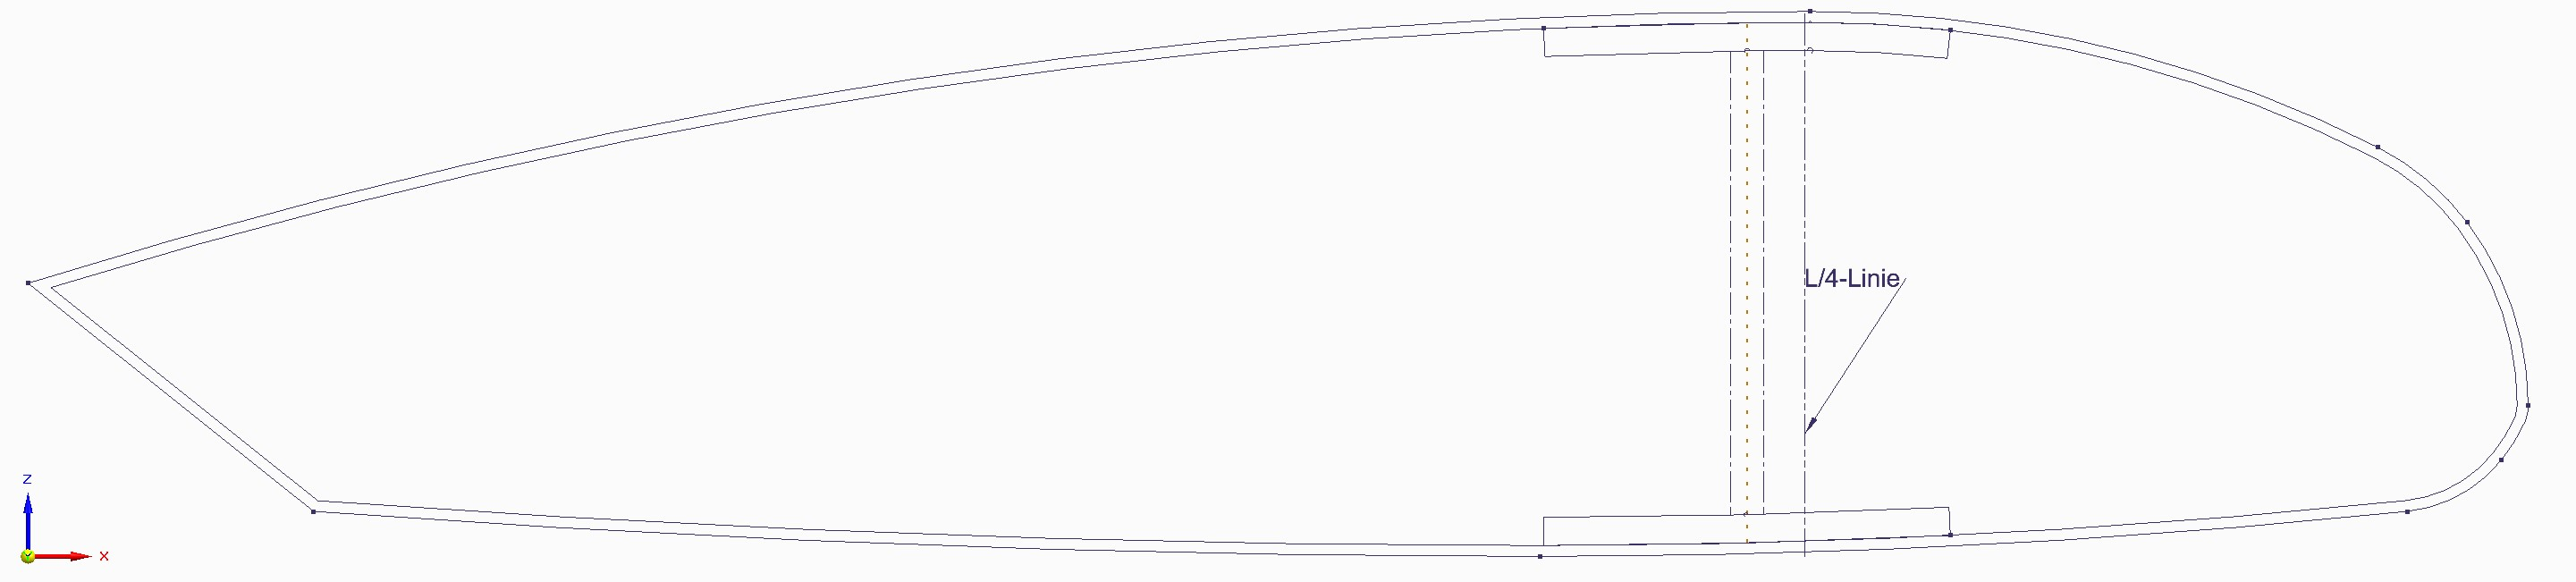
\includegraphics[width=1.0\textwidth]{Bilder/Kontur.jpg}
	\caption{Haut und Gurte nach dem ersten Schritt der Konstruktion in Solid Edge.}
	\label{fig: Kontur}
\end{figure} 
Der Vergleich mit dem erforderlichen Flächenträgheitsmoment zeigt, dass die angepasste Geometrie der Gurte die Steifigkeitsbedingung (vergleiche Beziehung ~\ref{IVergleich}) erfüllt. Die Haut konstanter Dicke und die Gurte im ersten Schritt der Konstruktion werden durch Abbildung ~\ref{fig: Kontur} veranschaulicht. Zusätzlich zeigt die Abbildung die ungefähre Lage der L/4-Linie. Diese wurde mithilfe einer vorhandenen Hilfsansicht der Tragfläche inklusive der Hinterkantenklappen und des Vorflügels, beide im eingefahrenen Zustand, ermittel. In der Hilfsansicht wird die abgebildete Länge des mittleren auszulegenden Teils der Tragfläche gemessen. Der Maßstab der Hilfsansicht bezüglich des Modellmaßstabes wird zu 1:2,529 berechnet. Diese Kenntnis ermöglicht die Berechnung des Abstandes der L/4-Linie zur Vorderkante der Haupttragfläche, der $ 42,2mm $ beträgt und besonders für die Berechnung der Torsion ausschlaggebend ist.\\

\begin{figure}[h]
	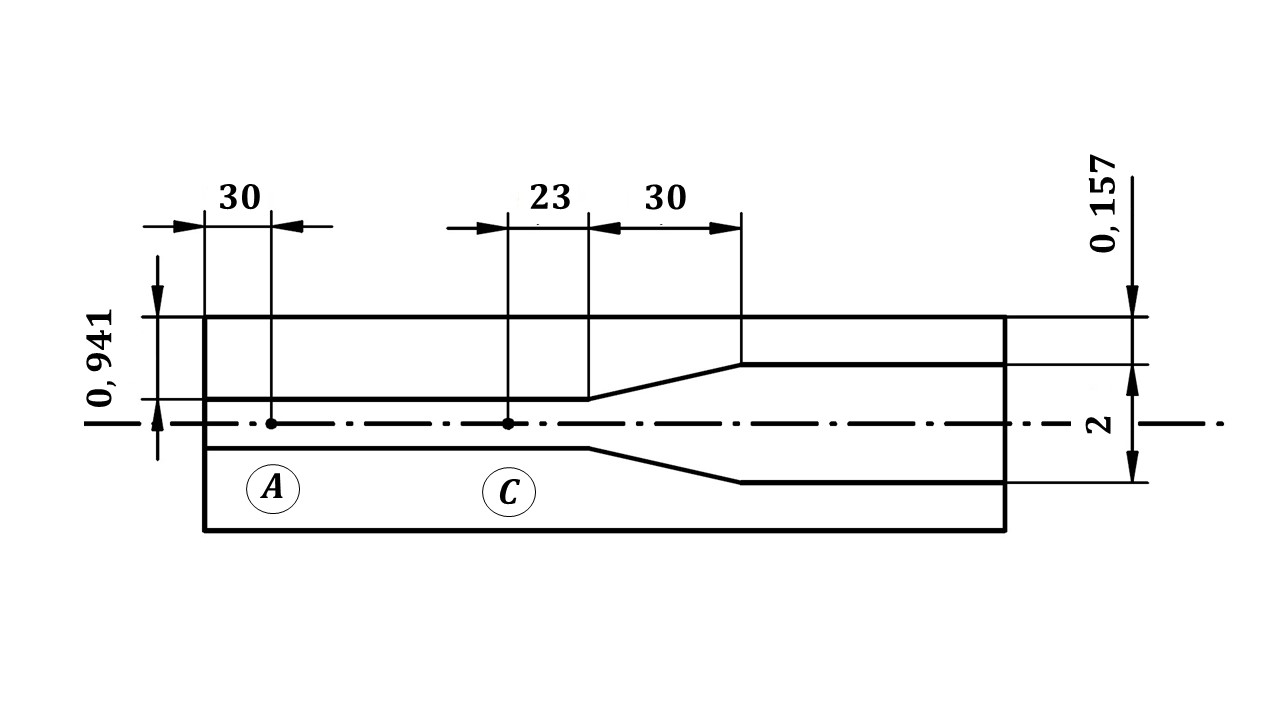
\includegraphics[width=1.0\textwidth]{Bilder/StegPrinzip.jpg}
	\caption{Prinzipskizze der Sandwichstruktur im Steg.}
	\label{fig: Steg}
\end{figure}



\subsection{Konstruktion des Stegs}

\noindent Im nächsten Schritt wird die Kontur der zwei Stegseiten und des Schaumes in einer weiteren Skizze über der Kontur der Gurte gezeichnet. Die vielschichtigen Skizzen erlauben den Bezug von Bauteilkanten aufeinander und erleichtern die spätere Extrusion der einzelnen Komponenten. So kann sichergestellt werden, dass in jeder Komponente der Bezug auf die umgebenden Tangentenbögen der Haut gewahrt bleibt. Die Konstruktion des Steges und des Schaumes erfordert auch die Berücksichtigung der verschieden belegten Unterteilungen des Stegs. Während der innere Teil des Stegs, am inneren freien Ende beginnend und $ 23mm $ über die Aufnahme der Querkraftbolzen an Punkt C hinweggehend, gemäß der Dimensionierung mithilfe des Laminatrechners mit 24 Lagen, aufgeteilt zu jeweils zwölf Lagen auf beiden Seiten des Schaums belegt wird, soll der gesamte äußere Teil mit nur insgesamt vier Lagen gleichmäßig verteilt belegt werden. Es bietet sich an, die vier Lagen des äußeren Teils über die gesamte Holmlänge zu erstrecken. Die 20 verstärkenden Lagen enden $ 23mm $ hinter Punkt C in einem sanften Übergang mit einer Länge von 30mm. Der dünn belegte Teil wird durch einen $ 2mm $ breiten Schaumkern vor dem Beulen geschützt, der zum dicken belegten Teil hin entsprechend schmaler wird. Das innere freie Ende wird auf eine Länge von $ 30mm $ im Abstand vom Mittelpunkt des Lagers A abgeschätzt. Abbildung ~\ref{fig: Steg} veranschaulicht den prinzipiellen Aufbau qualitativ.\\



\noindent Außerhalb des Bereichs der Gurte soll auch die Haut durch eine Sandwich-Konstruktion vor Beulen geschützt werden. In einem Abstand von $ 7mm $ neben den Gurten teilt sich die Haut in zwei Schichten auf. Die eine folgt der äußeren vorgegebenen Profilkontur, die andere verläuft auf der Innenseite des Schaumkerns. Zur Modellierung ohne die detaillierten Ergebnisse einer Auslegungsrechnung und Beulabschätzung der Haut wird eine gesamte Dicke von Schaumkern und Faserverbund von $ 3mm $ angenommen und mithilfe eines Offsets in dem CAD-Modell berücksichtigt. Der Übergang von aufeinanderliegenden Hautschichten zur Sandwichkonstruktion erfolgt auf einer Länge von $ 5mm. $\\



\noindent An den Enden des Bereichs 3 befinden sich die Wurzelrippe und die Endrippe. Beide werden nicht ausgelegt, es wird die Verwendung einer Sperrholzrippe ausreichender Stärke angenommen. Im CAD-Modell werden die Rippen auf einer neuen Skizze zwischen der Innenseite des Hautsanwich und der jeweiligen Seite der Holmes konstruiert. Der Holm teilt die Rippen in zwei Teile, beide Rippen wiederum sind gleich gestaltet, da sich die Profilform über die gesamte Länge des Flügels nicht ändert.


\noindent Im nächsten Schritt wird die Kontur der zwei Stegseiten und des Schaumes in einer weiteren Skizze über der Kontur der Gurte gezeichnet. Die vielschichtigen Skizzen erlauben den Bezug von Bauteilkanten aufeinander und erleichtern die spätere Extrusion der einzelnen Komponenten. So kann sichergestellt werden, dass in jeder Komponente der Bezug auf die umgebenden Tangentenbögen der Haut gewahrt bleibt. Die Konstruktion des Steges und des Schaumes erfordert auch die Berücksichtigung der verschieden belegten Unterteilungen des Stegs. Während der innere Teil des Stegs, am inneren freien Ende beginnend und $ 23mm $ über die Aufnahme der Querkraftbolzen an Punkt C hinweggehend, gemäß der Dimensionierung mithilfe des Laminatrechners mit 24 Lagen, aufgeteilt zu jeweils zwölf Lagen auf beiden Seiten des Schaums belegt wird, soll der gesamte äußere Teil mit nur insgesamt vier Lagen gleichmäßig verteilt belegt werden. Es bietet sich an, die vier Lagen des äußeren Teils über die gesamte Holmlänge zu erstrecken. Die 20 verstärkenden Lagen enden $ 23mm $ hinter Punkt C in einem sanften Übergang mit einer Länge von 30mm. Der dünn belegte Teil wird durch einen $ 2mm $ breiten Schaumkern vor dem Beulen geschützt, der zum dick belegten Teil hin entsprechend schmaler wird. Das innere freie Ende wird auf eine Länge von $ 30mm $ im Abstand vom Mittelpunkt des Lagers A abgeschätzt. Abbildung ~\ref{fig: Steg} veranschaulicht den prinzipiellen Aufbau qualitativ.

\begin{figure}[h]
	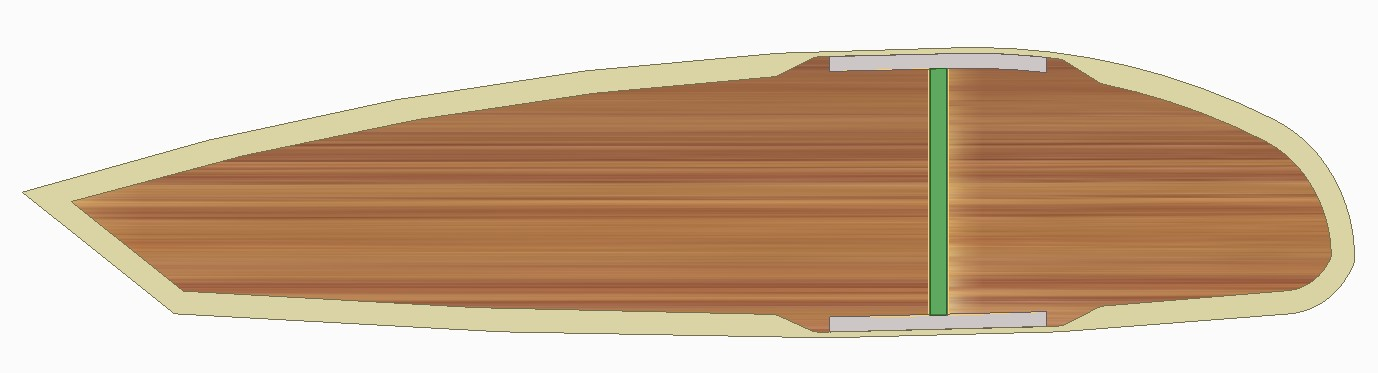
\includegraphics[width=1.0\textwidth]{Bilder/Seite.jpg}
	\caption{Seitenansicht auf die Endrippe}
	\label{fig: Seite}
\end{figure}

\subsection{Konstruktion der Haut und der Rippen}
Um die Haut vor Beulerscheinungen zu schützen, soll ein Schaumkern zwischen die innere und äußere Hautschicht gelegt werden. Zur ersten Modellierung wird eine gesamte Dicke der Sandwich-Konstruktion von $ 3mm $ angenommen. Diese Annahme soll nach erfolgter Auslegung der Haut nach Handbuchmethoden angepasst werden und dient zunächst allein der prinzipiellen Modellierung der Tragfläche in CAD. Um die Höhe $ h_{a} $ der Gurte möglichst nicht durch die Haut einzuschränken, soll der Schaumkern zu den Gurten hin in einem sanften Übergang auslaufen, sodass nur das Laminat über und unter den Gurten hergeführt werden muss. Abbildung ~\ref{fig: Seite} veranschaulicht die Gestaltung der Haut und den Übergang im Bereich der Gurte.\\

\noindent Der Freiraum zwischen Gurten, den Steglagen und der inneren Hautlage kann nun für die Vorder- und Hinterseite des Steges jeweils umrandet werden. Die darauf basierende Skizze ist die Grundlage der Konstruktion der zweigeteilten Wurzel- und Endrippe. Die Rippen werden in ihrer Dimensionierung als gegeben angenommen, eine Auslegung erfolgt im Rahmen dieser Projektarbeit nicht.\\

\subsection{Holzkonstruktion an der Aufnahme der Hauptbolzen}
Die Kraftaufnahme der  als Fest- und Loslager modellierten Punkte A und B erfolgt durch zwei Hauptbolzen, die im Flugzeug die Tragflächenhälften miteinander verbinden. In diesem Fall werden die Lagerkräfte von $ 5085N $ an den Teststand übertragen. Damit bei der Krafteinleitung in den Holm Spannungsspitzen vermieden werden, soll die Auflagefläche der Bolzen vergrößert werden. Dies geschieht, indem eine Holzkonstruktion für Vorder- und Rückseite des Holms erstellt wird, die der Kontur der Gurte angepasst ist und Bohrungen für die Bolzen enthält. Diese Klötzchen werden auf ihrer jeweiligen Stegseite mit den Gurten und dem Steg verklebt. Da der Abstand der Bohrungen mit $ 76mm $ gering ist, wird ein längeres Klötzchen für beide Bohrungen konstruiert. Aussparungen an den Seiten und zwischen den Bohrungen sollen das Gewicht der Klötzchen reduzieren. Die Konstruktion wird durch Abbildung ~\ref{fig: Klotz} veranschaulicht. Mit dem Positionieren der Bohrungen für die Hauptbolzen in dem Steg wird die Konstruktion abgeschlossen. Die Bohrungen befinden sich in der Mitte des Steges in z-Richtung in einem Abstand von $ l_{1} $ zueinander. $ l_{0} $ gibt die Positionierung in y-Richtung vor. 
\begin{figure}[h]
	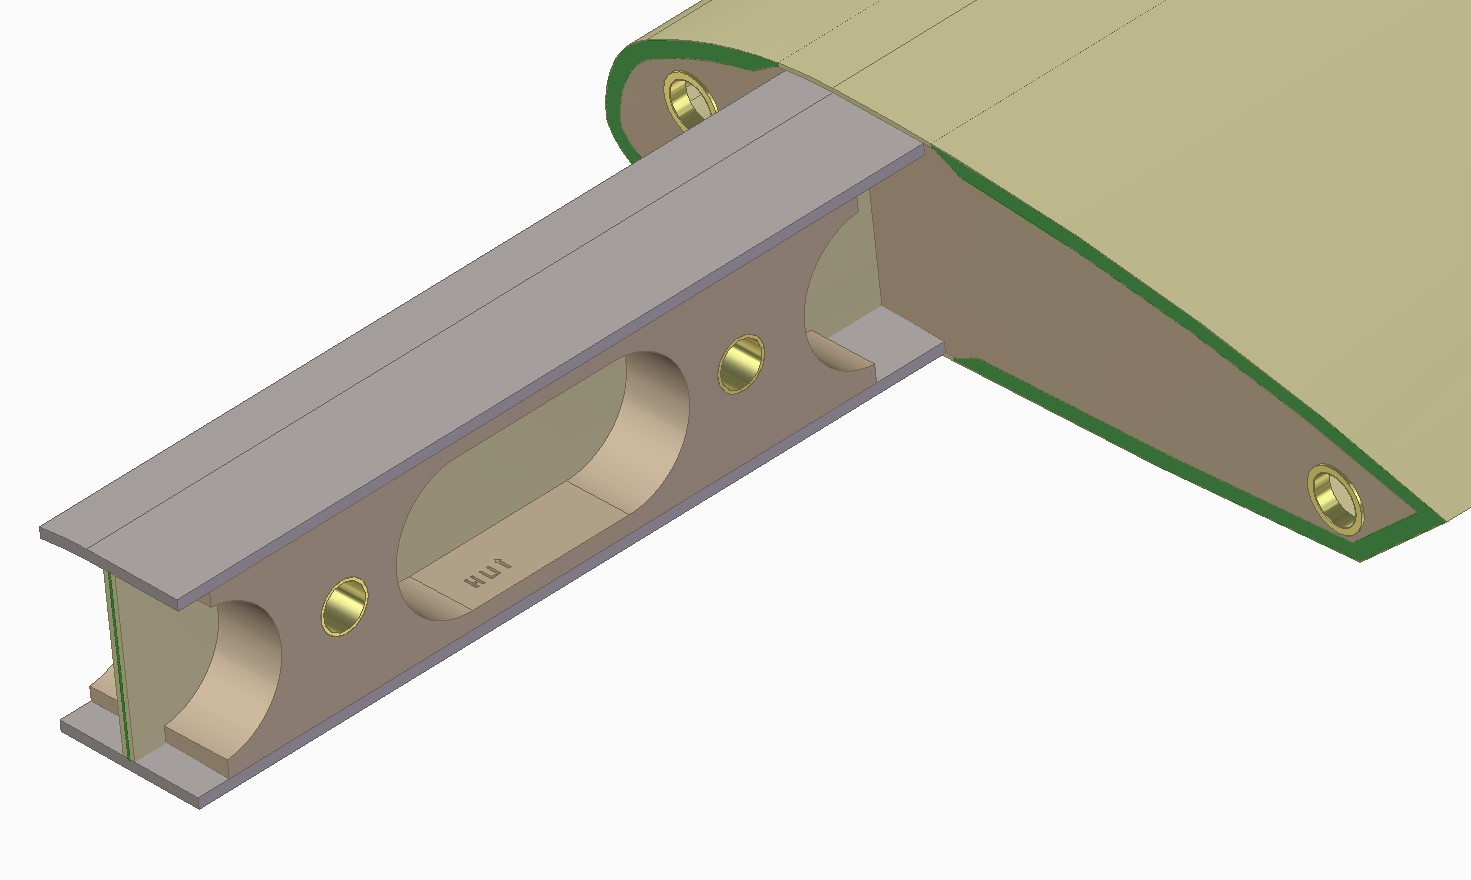
\includegraphics[width=1.0\textwidth]{Bilder/Klotz.jpg}
	\caption{Konstruktion der Holzklötze und Positionierung am Steg.}
	\label{fig: Klotz}
\end{figure}
